\documentclass[border = 5mm]{standalone}
%\documentclass[dvisvgm]{minimal}

\usepackage{tkz-euclide}

\usepackage[OT1]{fontenc}
\usepackage{sansmathfonts}

\begin{document}
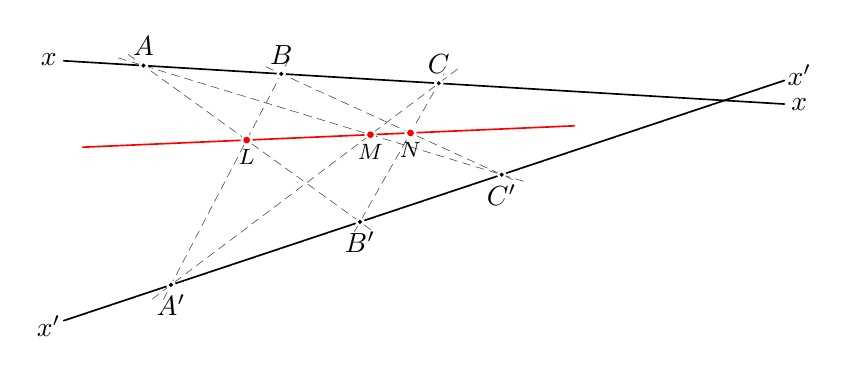
\begin{tikzpicture}

% Points A, B, and C on line x
\tkzDefPoints{0/0/X, 5/-0.3/Y}
\tkzDefPointOnLine[pos=0.05](X,Y)\tkzGetPoint{A}
\tkzDefPointOnLine[pos=0.4](X,Y)\tkzGetPoint{B}
\tkzDefPointOnLine[pos=0.8](X,Y) \tkzGetPoint{C}

% Points A', B', and C' on line x'
\tkzDefPoints{0/-3/X', 6/-1/Y'}
\tkzDefPointOnLine[pos=0.1](X',Y')\tkzGetPoint{A'}
\tkzDefPointOnLine[pos=0.5](X',Y')\tkzGetPoint{B'}
\tkzDefPointOnLine[pos=0.8](X',Y') \tkzGetPoint{C'}

% Draw x and x'
\tkzInterLL(X,Y)(X',Y') \tkzGetPoint{K}		
\tkzDrawLine[add = 0.1 and 0.1, semithick](X,K)
\tkzDrawLine[add = 0.1 and 0.1, semithick](X',K)

% Get L, M, N, the intersection points of AB' -- A'B, AC' -- A'C, BC' -- B'C
\tkzDrawLines[gray!150, add = 0.07 and 0.07, densely dashed, very thin](A,B' B,A' A,C' C,A' B,C' B',C)

\tkzInterLL(A,B')(A',B) \tkzGetPoint{L}
\tkzInterLL(A,C')(A',C) \tkzGetPoint{M}
\tkzInterLL(B,C')(B',C) \tkzGetPoint{N}

% Draw Line LN
\tkzDrawLines[red, add = 1 and 1, semithick](L,N)

% Label points and lines
\tkzDrawPoints[color=white, size=3](A,B,C,A',B',C')
\tkzDrawPoints[color=black, size=1](A,B,C,A',B',C') 

\tkzDrawPoints[color=white, size=4](L,M,N) 
\tkzDrawPoints[color=red, size=2](L,M,N) 

\tkzLabelPoints[above](A,B,C)
\tkzLabelPoints[below](A',B',C')
\tkzLabelPoints[font=\footnotesize](L,M,N)

\tkzLabelLine[pos=-0.125](X,K){$x$}     
\tkzLabelLine[pos=1.125](X,K){$x$}
\tkzLabelLine[pos=-0.125](X',K){$x'$}  
\tkzLabelLine[pos=1.125](X',K){$x'$}
		
\end{tikzpicture}
\end{document}